

\chapter{Bemessungsansatz für das Holz-Holzspanbeton-System}
In diesem Abschnitt wird der Vorschlag für ein Bemessungssystem für das Sandwichbauteil
Holz-Holspanbeton mit dem $\gamma$- Verfahren vorgestellt. Da noch Verbundversuche ausständig sind, welche die Einflüsse der Verbundwirkung genauer beschrieben, wird dieser Wert (Fugensteifigkeit: $c_{F}$) aus dem vorhandenen Versuch ermittelt. Weiters sind noch Langzeit-Untersuchungen am Bauteil zu machen, um das Kriechverhalten zu untersuchen. Die Berechnung sollte als Anstoß für ein Bemessungssystem dienen.\\

\subparagraph{Annahmen für das Beispiel:}

\begin{enumerate}
\item Es wird ein Plattenstreifen von $1m$ betrachtet.
\item Es wird eine gleichmäßige Flächenlast vorausgesetzt.
\item Das Sandwichsystem wird ausschließlich zur vertikalen Lastabtragung herangezogen.
\item Der Berechnung liegt ein statisch bestimmter Einfeldträger zu Grunde
\item konstante Querschnitte (max. drei Teilquerschnitte)
\end{enumerate}

\newpage

\section{Bauteilgeometrie und Abmessungen}

\begin{figure}[h!]
\begin{center}
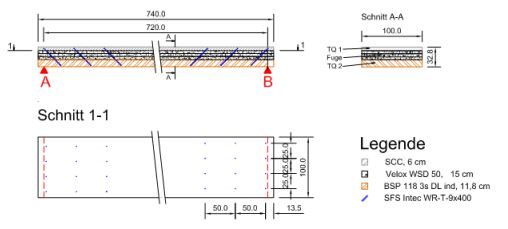
\includegraphics[scale =1.3]{Berechnungen/abbildungen/verbundplatte.JPG}
\caption{Beschriftung und Bemaßung der Verbungplatte}
\label{verbundplatte}
\end{center}
\end{figure}
\section{Angaben der Berechnung}

Die angeführten Werkstoffwerte sind dem Forschungsbericht "`Weitgespannte Flachdeckensysteme in Holzspanbeton - Verbundbauweise"' der TU Wien zu entnehmen.[]

\subsection{SVB}

\begin{align*}
\rho_{SCC}&=\unit[2400]{kg/m^{2}}\\
 f_{ck}&= \unit[30]{N/mm^{2}}\\
 E_{c}&= \unit[19560]{N/mm^{2}}\\
 f_{cd}&=\dfrac{f_{ck}}{\gamma_{M}}=\dfrac{32,79}{1,5}=\unit[21,86]{N/mm^{2}}
\end{align*}

\subsection{Velox}
\begin{align*}
\rho_{Velox}&=\unit[750]{N/mm^{2}}\\
G&=\unit[14,90]{N/mm^{2}}\\
f_{v.9090,k}&= \unit[0,28]{N/mm^{2}}\\
f_{v.9090,d}&=\dfrac{k_{mod} \cdot f_{v.9090,k}}{\gamma_{M}}=\dfrac{0,8 \cdot 0,28}{2}=\unit[0,11]{N/mm^{2}}\\ 
\end{align*}
\subsection{BSP}

Brettschichtholz: GLh24;NK1 \\
\begin{align*}
\rho_{CLT}&=\unit[470]{N/mm^{2}}\\
E_{0,mean}&=\unit[11600]{N/mm^{2}} \\
f_{m,k}&=\unit[24]{N/mm^{2}} \\
 f_{m,d}&=\dfrac{k_{mod} \cdot f_{m,d}}{\gamma_{M}}=\dfrac{24 \cdot 0,8}{1,5}=\unit[14,0]{N/mm^{2}}
\end{align*}


\section{Einwirkungen}


\begin{figure}[h!]
\caption{Berechnung des Eigengewichtes}
\begin{center}
\begin{tabular}{|c|c|c|c|}
\hline 
Schichtenfolge & $\rho$ $[kg/m^{3}]$ & Volumen $[m^{3}]$ &  Eigengewicht $[kN/m] $\\ 
\hline 
 1 Schicht (SCC) & 2400 & 0,43 & 1,41 \\ 
\hline 
Fuge (Velox) & 750 & 1,08 & 1,10 \\ 
\hline 
2 Schicht (CLT) & 470 & 0,85 & 0,55 \\ 
\hline\hline 
Summe &  &  & 3,06 \\ 
\hline 
\end{tabular} 
\end{center}
\end{figure}

\begin{align*}
Eigengewicht: g_{k1}&=\unit[3,06]{kN/m}\\
Bodenaufbau: g_{k2}&= \unit[1,60]{kN/m}\\
Nutzlast:q_{k}&=\unit[3,0]{kN/m}\\
\gamma_{M1}&=\unit[1,35]{} \\
\gamma_{M2}&=\unit[1,50]{} \\
 \end{align*}

\begin{align*}
q_{d}&= \gamma_{M1} \cdot (g_{k1}+g_{k2})+\gamma_{M2} \cdot q_{k}=\\
p_{d}&=1,35 \cdot (3,06 + 1,60)+1,50 \cdot 3,0=\unit[10,79]{kNm}
\end{align*}
\section{Bemessungsschnittgrößen}
\begin{align*}
M_{d}&=\dfrac{p_{d} \cdot l^{2}}{8}=\dfrac{10,79 \cdot 7,20^{2}}{8}= \unit[69,92]{kNm}\\
V_{d}&=\dfrac{p_{d} \cdot l}{2}=\dfrac{10,79 \cdot 7,20}{2}=\unit[38,84]{kN}
\end{align*}

\section{Verschiebungsmodul}

Fugensteifigkeit: $c_{F}=\unit[260]{MN/m^{2}}$ wurde aus dem Versuch zurückgerechnet???????

\begin{align*}
c_{F,d}= \dfrac{c_{F}}{\gamma_{M}}=\dfrac{260}{1,5}=\unit[173,33]{MN/m^{2}}
\end{align*}

\section{Bestimmung der effektiven Biegesteifigkeit}
\unit[]{}
\begin{figure}[h!]
\caption{Berechnung der Querschnittswerte der Teilquerschnitte}
\begin{center}
\begin{tabular}{|c|c|c|c|c|c|}
\hline 
Schichtenfolge & $A=b*h_{i}$ & $I_{i}=\dfrac{b \cdot h_{i}^{3}}{12}$ & $E_{i}\cdot A_{i}$ & $E_{i}I_{i}$  \\ 

& $[cm^{2}]$ & $[cm^{4}]$ & $[MN]$ & $[MN \cdot m^{2}]$  \\ \hline 
\hline
1 Schicht (SCC) & 600 & $1,80 \cdot 10^{3}$ & $1,17 \cdot 10^{3}$ & 0,35  \\ 
\hline 
Fuge (Velox) & 1500 & $2,81  \cdot 10^{4}$ &  &   \\ 
\hline 
2 Schicht (CLT) & 1180 & $1,37 \cdot 10^{4}$ & $1,37 \cdot 10^{3}$ & 1,58  \\ 
\hline 
\end{tabular} 
\end{center}
\end{figure}


\subsection{Bestimmug der $\gamma$ Faktoren}
\begin{align*}
\gamma_{1}&=\dfrac{1}{1+\dfrac{\Pi^{2} \cdot E_{1} \cdot A_{1}}{c_{F} \cdot l^{2}}}=\dfrac{1}{1+\dfrac{\pi^{2} \cdot 1,1754 \cdot 10^{3}}{260 \cdot 7,20^{2}}}= \unit[0,538]{}\\\\
\gamma_{2}&=\unit[1,0]{}
\end{align*}



\subsection{Bestimmung des Schwerpunktes}
\begin{align*}
a&=\dfrac{h_{1}+h_{2}}{2}+t_{F}=\dfrac{0,06+0,118}{2}+0,15= \unit[0,239]{m}\\\\
a_{2}&=\dfrac{\gamma_{1}*E_{1}A_{1}*a}{\gamma_{1} \cdot E_{1}A_{1} \cdot E_{2}A_{2}}=\dfrac{0,538 \cdot 1,174 \cdot 10^{3} \cdot 0,239}{0,538 \cdot 1,174 \cdot 10^{3} \cdot 1,369 \cdot 10^{3}}= \unit[0,076]{m}\\\\
a_{1}&=a-a_{2}=0,239-0,076=\unit[0,163]{m}\\
\end{align*}
\subsection{Bestimmung der effektiven Biegesteifigkeit}
\begin{align*}
EI_{eff}&=E_{1}I_{1}+E_{2}I_{2}+\dfrac{a^{2} \cdot \gamma_{1} \cdot E_{1}A_{1} \cdot E_{2}A_{2}}{\gamma_{1} \cdot E_{1}A_{1}+E_{2}A_{2}}= \\
EI_{eff}&=0,352+1,588+\dfrac{0,239^{2} \cdot 0,538 \cdot 1,174 \cdot 10^{3} \cdot 1,369 \cdot 10^{3}}{0,538 \cdot 1,174 \cdot 10^{3}+1,369 \cdot 10^{3}}= \unit[13,34]{MN/m^{2}} \\
\end{align*}

\section{Schnittgrößen der Teilquerschnitte}

\subparagraph{Teilquerschnitt 1}
\begin{align*}
N_{1}&=-\dfrac{M_{d}}{EI_{eff}} \cdot \gamma_{1} \cdot a_{1} \cdot E_{1}A_{1}=-\dfrac{69,92}{13,34} \cdot 0,538 \cdot 0,163 \cdot 1,174 \cdot 10^{3}=\unit[-271,22]{kN}\\
M_{1}&=\dfrac{M_{d}}{EI_{eff}} \cdot E_{1}I_{1}=\dfrac{69,92}{13,34} \cdot 0,352= \unit[0,925]{kNm}\\
\end{align*}

\subparagraph{Teilquerschnitt 2}
\begin{align*}
N_{2}&=\dfrac{M_{d}}{EI_{eff}} \cdot \gamma_{2} \cdot a_{2} \cdot E_{2}A_{2}=\dfrac{69,92}{13,34} \cdot  1,0 \cdot 0,076 \cdot 1,369 \cdot 10^{3}= kN\unit[271,22]{kN} \\
M_{2}&=\dfrac{M_{d}}{EI_{eff}} \cdot E_{2}I_{2}=\dfrac{69,92}{13,34} \cdot 1,588=\unit[4,17]{kNm}\\
\end{align*}


\section{Ermittlung der Normalspannungen}
\subparagraph{Teilquerschnitt 1}
\begin{align*}
\sigma_{1,o,d}&=\dfrac{N_{1}}{A_{1}}-\dfrac{M_{1}}{I_{1}} \cdot \dfrac{h_{1}}{2}=\dfrac{-271,22}{0,06}-\dfrac{0,952}{0,18 \cdot 10^{-4}}*\dfrac{0,06}{2}=  \unit[-6,062]{N/mm^{2}}\\\\
\sigma_{1,u,d}&=\dfrac{N_{1}}{A_{1}}+\dfrac{M_{1}}{I_{1}} \cdot \dfrac{h_{1}}{2}=\dfrac{271,22}{0,06}+\dfrac{0,952}{0,18*10^{-4}} \cdot \dfrac{0,06}{2}= \unit[-2,979]{N/mm^{2}}
\end{align*}

\subparagraph{Teilquerschnitt 2}
\begin{align*}
\sigma_{2,o,d}&=\dfrac{271,22}{0,118}-\dfrac{4,172}{I_{2}} \cdot \dfrac{h_{2}}{2}=\dfrac{N_{2}}{A_{2}}-\dfrac{M_{2}}{I_{2}} \cdot \dfrac{h_{2}}{2}=\unit[0,501]{N/mm^{2}}\\\\
\sigma_{2,u,d}&=\dfrac{271,22}{0,118}+\dfrac{4,172}{1,369 \cdot 10^{4}} \cdot \dfrac{0,118}{2}=\dfrac{N_{2}}{A_{2}}+\dfrac{M_{2}}{1,369 \cdot 10^{4}} \cdot \dfrac{0,118}{2}=\unit[4,092]{N/mm^{2}}
\end{align*}



\begin{figure}[h!]
\begin{center}
\begin{tikzpicture}
\begin{axis}[	height=8cm, width=8cm,no markers,
				ylabel=h \,$\lbrack cm \rbrack $ ,
				ymin=0,axis y line=center,
				xlabel=$\sigma$\,$\lbrack MN/m^2\rbrack $,
				xmin=-7, xmax=7, 													
				legend pos= outer north east	
			]
			\addplot table[y=hsigma,x=sigma]{Berechnungen/abbildungen/versuch3.dat};
			\legend{Normalspannung}
\end{axis}
\end{tikzpicture}
\caption{Normalspannungsverlauf im Gesamtquerschnitt}
\label{normalspannungen}
\end{center}
\end{figure}







\section{Ermittlung der Schubspannungen}
\subparagraph{Teilquerschnitt 1}



\begin{align*}
\tau_{1,o,d}& =\unit[0,0]{N/mm^{2}}\\\\
\tau_{1,u,d}& =\dfrac{\gamma_{1} \cdot E_{1}A_{1} \cdot a_{1} \cdot V_{d}}{EI_{eff} \cdot b}= \dfrac{0,538 \cdot 1,174 \cdot 10^{3} \cdot 0,163 \cdot 38,84}{13,341 \cdot 1,0}= \unit[0,151]{N/mm^{2}}\\
\end{align*}

\subparagraph{Teilquerschnitt 2}
\begin{align*}
\tau_{2,o,d}& =\dfrac{0,5 \cdot E_{2} \cdot (\dfrac{h_{2}}{2}+a_{2})^{2} \cdot V_{d} }{EI_{eff}}=\dfrac{0,5 \cdot 11600 \cdot (\dfrac{0,118}{2}+0,076)^{2} \cdot 38,84}{13,341}=\unit[0,153]{N/mm^{2}}\\\\
\tau_{2,u,d}& =\unit[0,0]{N/mm^{2}}\\
\end{align*}



\begin{figure}
\begin{center}
\begin{tikzpicture}
\begin{axis}[	legend pos= outer north east,
				height=8cm, width=8cm,
				no markers,
				ylabel=h \,$\lbrack cm \rbrack $  ,
				ymin=0,xmin=0,
				xlabel=$\tau$\,$\lbrack MN/m^2\rbrack $
				]
				
				\addplot table[y=htau,x=tau]{Berechnungen/abbildungen/versuch3.dat};
				\legend{Schubspannung}
\end{axis}
\end{tikzpicture}
\caption{Schubspannungsverlauf nach dem $\gamma$- Verfahren, über den Querschnitt}
\label{schubspannung}
\end{center}
\end{figure}


\section{Spannungsnachweise}

\subparagraph{SCC}

\begin{align*}
\dfrac{\sigma_{1,o,d}}{f_{m,d}}&=\dfrac{6,06}{20,86}=\unit[0,18]{} < \unit[1,0]{}\\\\
\dfrac{\sigma_{1,o,d}}{f_{m,d}}&=\dfrac{2,98}{20,86}=\unit[0,14]{} < \unit[1,0]{}\\\\
\dfrac{\tau_{1,o,d}}{f_{90}}&=
\end{align*}

\subparagraph{Velox}

\begin{align*}
\dfrac{\tau_{max}}{f_{v,9090,d}}&=\unit[1,39]{} > \unit[1,0]{}
\end{align*}
\subparagraph{SCC}

\begin{align*}
\dfrac{\sigma_{2,o,d}}{f_{m,d}}&=\dfrac{0,50}{14,0}=\unit[0,04]{} < \unit[1,0]{}\\\\
\dfrac{\sigma_{2,o,d}}{f_{m,d}}&=\dfrac{4,10}{14,0}=\unit[0,29]{} < \unit[1,0]{}\\\\
\dfrac{\tau_{2,o,d}}{f_{90}}&=
\end{align*}

\section{Durchbiegung}

\subparagraph{Durchbiegung zufolge Eingengewicht}

\begin{align*}
w_{g}&=\dfrac{5 \cdot (g_{k1}+g_{k2}) \cdot l^{4} }{384 \cdot EI_{eff} }=\dfrac{5 \cdot (3,06 + 1,60) \cdot 7,20^{4} }{384 \cdot 13,41}=\unit[6,13]{mm} 
\end{align*}

\subparagraph{Durchbiegung zufolge Nutzlast}

\begin{align*}
w_{p}&=\dfrac{5 \cdot p_{k}\cdot l^{4} }{384 \cdot EI_{eff} }=\dfrac{5 \cdot 3,0 \cdot 7,20^{4} }{384 \cdot 13,41}= \unit[3,94]{mm}
\end{align*}

\subparagraph{Charakteristische Bemessungssituation:Anfangszustand}

\begin{align*}
w_{Q,inst}&\leq\dfrac{l}{300}=\dfrac{7200}{300}=\unit[24,0]{mm}\\
w_{Q,inst}&=\unit[3,94]{mm}\leq \unit[24,0]{mm}
\end{align*}


\subparagraph{Charakteristische Bemessungssituation:Endzustand}

\begin{align*}
w_{fin}-w_{G,inst}&\leq\dfrac{l}{200}=\dfrac{7200}{200}=\unit[36,0]{mm}\\
w_{fin}-w_{G,inst}&=w_{G,inst}+\sum_{i\geqslant1} w_{Q,i,inst} \cdot \psi_{0,i}(w_{G,inst}+\Psi_{2,1} \cdot w_{Q,1,inst}+\sum w_{Q,i,inst} \cdot \Psi_{2,1}) \cdot k_{def}\\
w_{fin}-w_{G,inst}&=3,94+0+(6,13+0,3\cdot 3,94+0) \cdot 0,6=\unit[8,32]{mm} < \unit[36,0]{mm}
\end{align*}

\subparagraph{Quasi-ständige Durchbiegung:Endzustand}
\begin{align*}
w_{fin}-w_{c}&\leq\dfrac{l}{250}=\dfrac{7200}{250}=28,8mm\\
w_{fin}-w_{c}&=(w_{G,inst}+\sum_{i\geqslant1} \Psi_{2,1} \cdot w_{Q,i,inst}) \cdot (1+k_{def})-w_{c}=\\
w_{fin}-w_{c}&=(6,13+0,3 \cdot 3,94) \cdot (1+0,6)-0=\unit[11,70]{mm} < \unit[28,80]{mm}
\end{align*}






